\section{Working Resources Area}
The Working Resource Area encompass all the AllSpark's business processes that characterize its right lifecycle and functionalities releated to the working environment. Each business process aims to satisfy some specific objective needed by correctness and the efficiency of processes in other areas, but that are not required in advance for the productivity roles the Company wants to achieve. The employees involved in the business processes are potentially of all kind foreseen in the Working Structure presented in figure \ref{2img:working}.

A particular observation is reserved to the responsibility role of this Area. Since each area has a responsible the discussion about it is relavant, but not so simple to define a unique responsible except for the CEO; generally is defined an Area Manager that leads all the business processes, but pratically is more efficient that each process is assigned to the most similar manager.

The business process Systems management has not been modeled since is very general and most of its processes are not really interesting.

\subsection{Updating Management}
This Updating Management business process is derived by the macro business process ``Systems Management'' that provides, as the name suggests, the service of ``up to date'' systems meaning softwares, both products and tools, and hardwares in order to minimize the presence of bugs, improve the efficiency and acquire new features.

The main responsible of this business process is the System Manager who has the very important role of manage all the tasks reducing the possible side effects. For certain task the System Manager is not required to be responsible since are not warning activities. The whole process is shown in figure \ref{2img:updating}.

\begin{figure}[ht!]
\begin{centering}
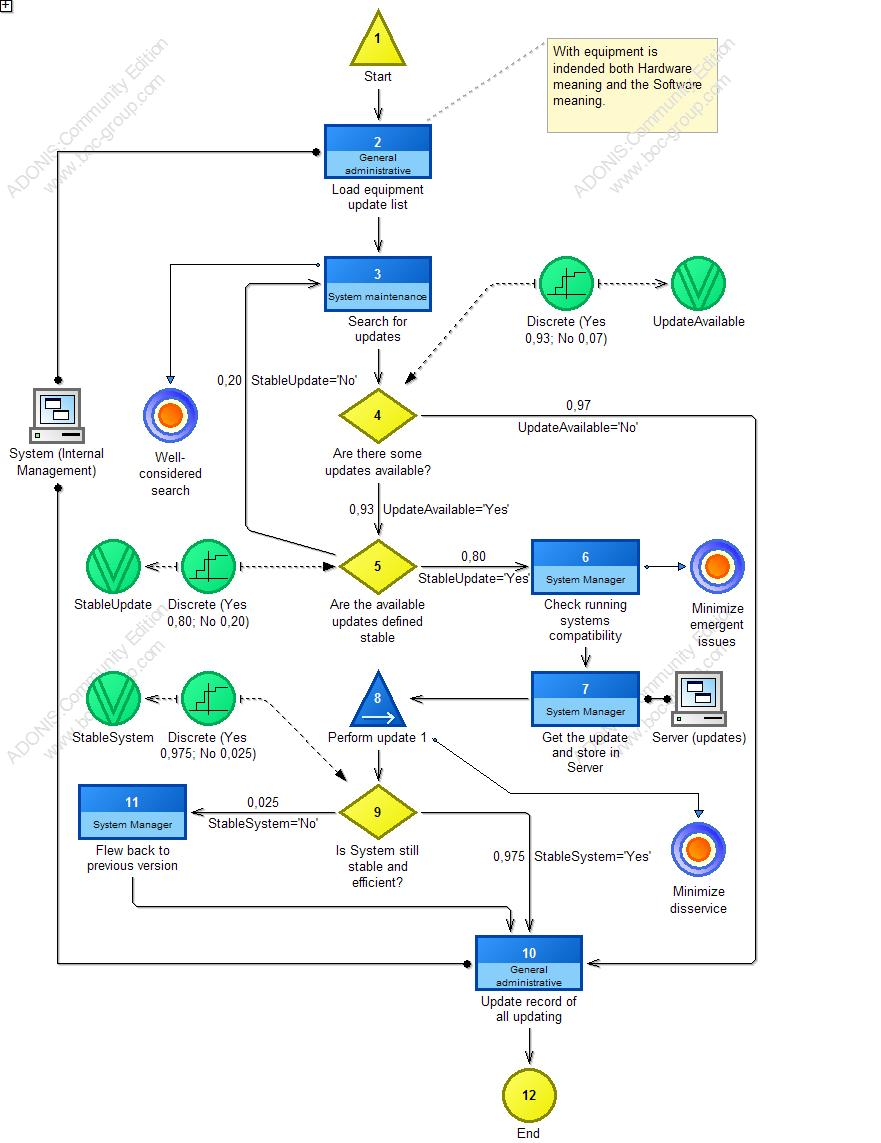
\includegraphics[scale=0.50]{assign2/adonis/imgs/updating.jpg}
\caption{AllSpark Updating Management.}
\label{2img:updating}
\end{centering}
\end{figure}


\subsubsection{Path Analysis}
According to the results of path analysis, an update is expected to succeed with the probability of 73,70\% as foreseen. The whole process is quite cheaper and the time is considered with nothing going badly. The following report returns the complete information about it.

\begin{alltt}
Probability:   73,7000\%
Execution time:  00:000:01:21:00
Waiting time:  00:000:00:02:00
Resting time:  00:000:00:12:00
Transport time:  00:000:00:10:00
Cycle time:  00:000:01:45:00
Costs:  1,980000

Updating Management 0.3 (Business process model)
========================================
Process start: Start
Activity: Load equipment update list
Activity: Search for updates
Decision: Are there some updates available? --> UpdateAvailable='Yes'
Decision: Are the available updates defined stable --> StableUpdate='Yes'
Activity: Check running systems compatibility
Activity: Get the update and store in Server
Subprocess: Perform update
Decision: Is System still stable and efficient? --> StableSystem='Yes'
Activity: Update record of all updating
End: End

Updating Management 0.3 (Business process model) --> Perform update 1 (Business process model)
========================================
Process start: Start
Activity: Perform update
End: End
\end{alltt}


\subsubsection{Capacity Analysis}
The capacity analysis for this process shows the interesting activites' report which are strongly dependent by the System Manager which is represented by either Sysadmin or Area Manager distinguishing the cases in which he is the real responsible of the entire AllSpark's system structure.

\begin{landscape}
\begin{table}
\centering
{\tiny
\begin{tabular}{|l|l|l|l|l|l|l|}
Business process&Activity&Performer&Number&Execution time&Cycle time&Costs\\
\hline
Updating Management 0.3&&&&00:000:01:23:33&00:000:01:48:07&5,966800\\
\hline
&Load equipment update list &&1,000000&00:000:00:01:00&&0,200000\\
\hline
&&Secretary &1,000000&00:000:00:01:00&&0,200000\\
\hline
&Update record of all updating &&1,000000&00:000:00:15:00&&0,900000\\
\hline
&&Secretary &1,000000&00:000:00:15:00&&0,900000\\
\hline
&Search for updates &&1,240000&00:000:00:24:48&&0,248000\\
\hline
&&Sysadmin &1,240000&00:000:00:24:48&&0,248000\\
\hline
&Check running systems compatibility &&0,910000&00:000:00:09:06&&0,273000\\
\hline
&&Area Manager &0,910000&00:000:00:09:06&&0,273000\\
\hline
&Flew back to previous version &&0,020000&00:000:00:01:48&&4,000000\\
\hline
&&Area Manager &0,020000&00:000:00:01:48&&4,000000\\
\hline
&Get the update and store in Server &&0,910000&00:000:00:13:39&&0,273000\\
\hline
&&Area Manager &0,910000&00:000:00:13:39&&0,273000\\
\hline
&Perform update &&0,910000&00:000:00:18:12&&0,072800\\
\hline
&&Sysadmin &0,910000&00:000:00:18:12&&0,072800\\
\hline
Total&&&&00:000:01:23:33&&5,966800
\end{tabular}
}
\caption{Capacity analysis for Updating Management.}
\end{table}
\end{landscape}
%

%

\subsection{Security checking}
The ``Security checking'' business process scope is to achieve the best protection through prevention against introuders, external penetration attempts, system's robustness and security, reliability with high load application and stability. To performing all the test, sometime is necessary to require a professional\footnote{In particular penetration test are aimed by AllSpark to certificate its quality.} that has experience in this kind of application and, over all, that is costantly up to date with respect to the always new method to trick the barriers.

Since the test concern both implemented product and the acquired product, the main responsible of all the operation is located on the Project management role which sorround all the aspect of the Company's system. The testing functionalities are followed also by some element of ``Research & Development'' organizational unit represented in figure \ref{2img:working}.

\begin{figure}[ht!]
\begin{centering}
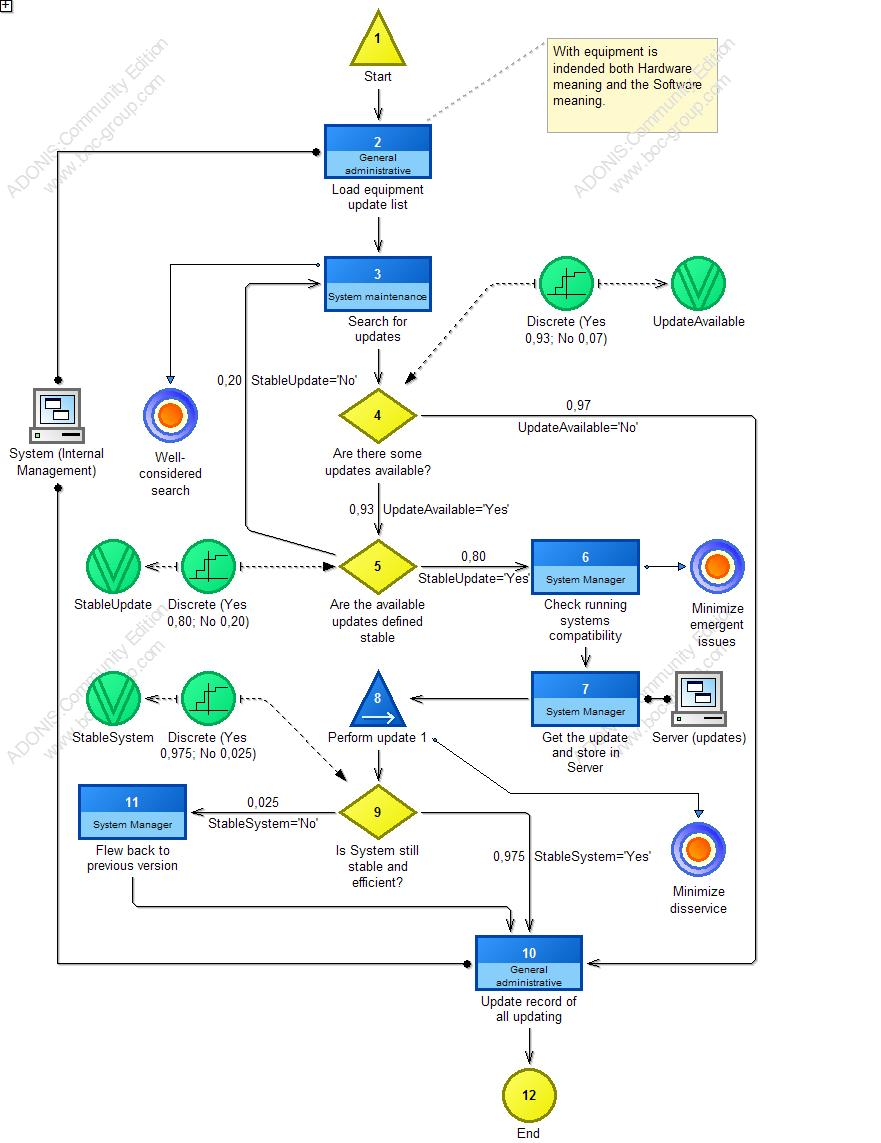
\includegraphics[scale=0.50]{assign2/adonis/imgs/updating.jpg}
\caption{AllSpark Updating Management.}
\label{2img:updating}
\end{centering}
\end{figure}


\subsubsection{Path Analysis}


\begin{alltt}

\end{alltt}


\subsubsection{Capacity Analysis}


\begin{landscape}
\begin{table}
\centering
{\tiny
\begin{tabular}{|l|l|l|l|l|l|l|}
Business process&Activity&Performer&Number&Execution time&Cycle time&Costs\\
\hline

\end{tabular}
}
\caption{Capacity analysis for Updating Management.}
\end{table}
\end{landscape}
%

%